\documentclass{article}
\usepackage{graphicx}
\usepackage{geometry}
\usepackage{hyperref}
\usepackage{mathtools}
\usepackage{float}
\usepackage{minted}
\usepackage{xcolor}
\definecolor{LightGray}{rgb}{0.85,0.85,0.85}
\graphicspath{{./}}
\geometry{a4paper, portrait, margin = 1in}
\title{ROS Made Easy \\6: ROS Control}
\date{\today}
\author{Aniruddh K Budhgavi \\Enigma, IIIT-B}
\begin{document}
    \maketitle
    \section{Notes}
    \begin{enumerate}
        \item This tutorial was created for \textbf{ROS1 Melodic Morenia}
        on \textbf{Ubuntu 18.04 Bionic Beaver}, in \textbf{June 2020}.
        I expect them to become rapidly out of date. It is my hope
        that Team Enigma will continually maintain and update these tutorials.
        \item This tutorial assumes that you are running Ubuntu, and have at least an
        elementary grasp of Python 2.7 and C/C++ .
        \item All the code and the models for this tutorial are available at 
        \url{https://github.com/aniruddhkb/enigmatutorials}.
        \item The aim of this tutorial is to make you \emph{functional} in ROS, not to make you a master. For 
        that, look elsewhere.
        \item Ensure that you have RViz, TF2, the robot\_state\_publisher package and the joint\_state\_publisher
        and joint\_state\_publisher\_gui packages installed before proceeding further. You can install them 
        using the relevant \texttt{apt-get} commands. See \url{http://wiki.ros.org/rviz/UserGuide},
        \href{http://wiki.ros.org/tf2/Tutorials/Introduction%20to%20tf2}{this} and
        \href{https://answers.ros.org/question/346665/how-to-install-joint_state_publisher_gui-in-melodic-version-of-ros/}{this}.

        \item Ensure that you have \textbf{Meshlab} installed. Get it \href{https://snapcraft.io/install/meshlab/ubuntu}{here}.
        
        \item Ensure that you have the \textbf{ros\_control} and \textbf{ros\_controllers} packages installed. Get them \href{http://wiki.ros.org/ros_control#Install}{here}.
    \end{enumerate}
    \section{Introduction}
        \begin{enumerate}
            \item ROS provides an interface for controlling robot joints. These interfaces are fairly sophesticated -- they provide a reasonable 
            amount of feedback control. However, the documentation quality leaves something to be desired for beginners. Make yourself familiar with the 
            contents of \url{http://wiki.ros.org/ros_control} and \url{http://gazebosim.org/tutorials/?tut=ros_control} before you begin this tutorial. Also ensure 
            that you have the packages mentioned above.
            \item Gazebo's tutorials page provides the following diagram to explain how the ROS interface and the 
            Gazebo ROS control plugin work together.
            \begin{figure}[H]
                \center
                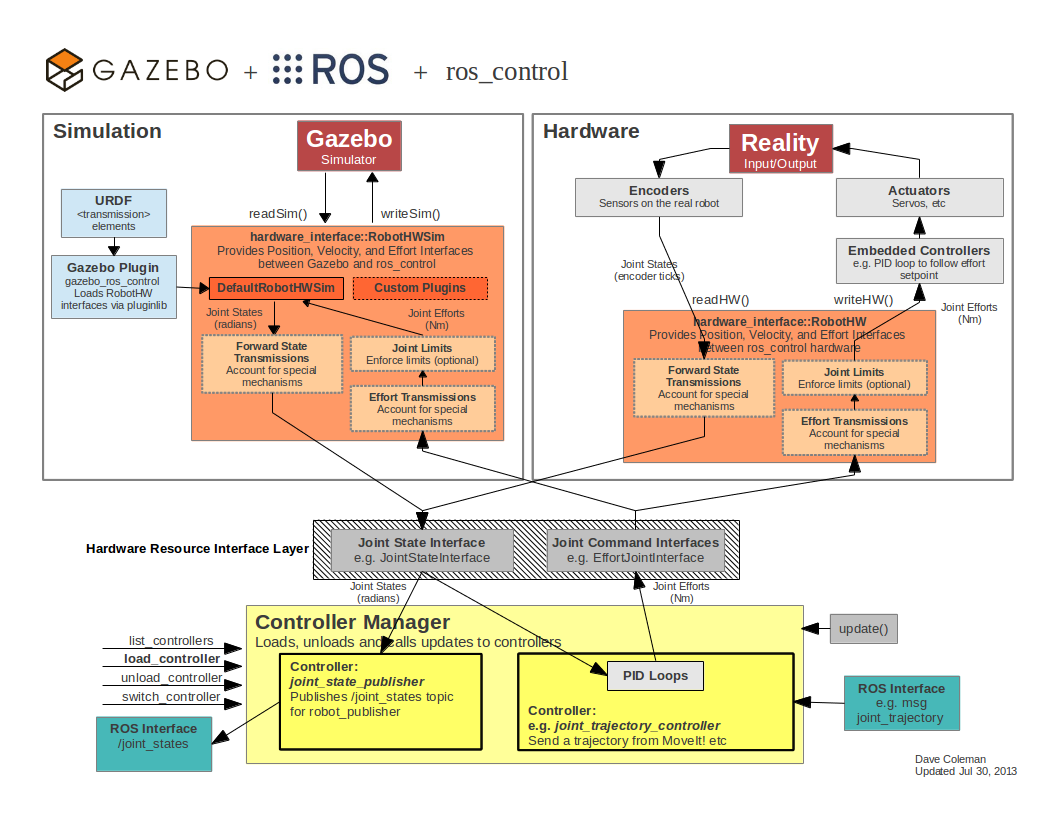
\includegraphics[width = \textwidth]{image_1.png}
            \end{figure}
            Let's break it down.
            \begin{enumerate}
                \item We have the Gazebo simulator, the URDF file and the Gazebo ROS control plugin.
                \item The Gazebo ROS control plugin sets up simulated hardware interfaces between ROS and Gazebo.
                These interfaces provide communication between Gazebo and the ROS controllers. They write and 
                read from the sim, accept commands from the ROS interfaces and provide the feedback to the ROS 
                interface. They also enforce joint limits, like the position, velocity and effort limits.
                \item The hardware interface set up by ROS is the hub of ROS control. \emph{Theoretically}, it 
                should be possible to use the same code to control the simulated robot and the real robot. Of course,
                there are some complications in this.
                \item The ROS controller manager handles the controllers. You can publish messages to this manager's topics
                 to control the robot and you can get joint state information from this manager.
                 This is also where the PID control loops are set up.
            \end{enumerate}
        \end{enumerate}
    \section{Enabling ROS control}
        \subsection{Modifying the URDF}
            \begin{enumerate}
                \item Take the URDF from the last tutorial and add the following lines between the 
                \texttt{robot} tags. \newpage
                \begin{minted}[bgcolor=LightGray]{xml}
<transmission name = "t1">
  <type>
    transmission_interface/SimpleTransmission
  </type>
  <joint name="j1">
    <hardwareInterface>
      hardware_interface/PositionJointInterface
    </hardwareInterface>
  </joint>
  <actuator name="a1">
    <mechanicalReduction>1</mechanicalReduction>
  </actuator>
</transmission>
<transmission name = "t2">
  <type>
    transmission_interface/SimpleTransmission
  </type>
  <joint name="j2">
    <hardwareInterface>
      hardware_interface/PositionJointInterface
    </hardwareInterface>
  </joint>
  <actuator name="a2">
    <mechanicalReduction>1</mechanicalReduction>
  </actuator>
</transmission>
<gazebo>
  <plugin name = "gazebo_ros_control" 
          filename="libgazebo_ros_control.so"/>
</gazebo>                    
                \end{minted}
                Line-by-line:
                \begin{enumerate}
                    \item The \texttt{transmission} tag is to set up the interfaces.
                    \item There is only one \texttt{type} supported in Gazebo.
                    \item The \texttt{hardwareInterface} corresponds to the intermediate layer which 
                    is used to communicate with the joints (both real and simulated). The full 
                    list of supported hardware interfaces is \href{http://wiki.ros.org/ros_control#Hardware_Interfaces}{here}.
                    The important ones are:
                    \begin{itemize}
                        \item \textbf{Effort Joint Interface}: To pass effort commands to the joint.
                        \item \textbf{Position Joint Interface}: To pass position commands to the joint.
                        \item \textbf{Velocity Joint Interface}: To pass velocity commands to the joint.
                    \end{itemize}
                        All three interfaces mentioned above can accept effort, position and velocity commands 
                        from the controller manager. What changes is what commands they pass to the joints.
                        Another important interface is 
                    \begin{itemize}
                        \item \textbf{Joint State Interface}: To pass the data of the current joint positions, velocities and
                        efforts to ROS in the form of arrays.
                    \end{itemize}
                    \textbf{Note:} The ROS and Gazebo tutorials erroneously mention that only Effort Joint Interface is 
                    supported in Gazebo. This information is out-of-date. I have successfully used both Position and Velocity interfaces 
                    in Gazebo, and will be showing you how to do the same in this and the next tutorial.

                    \item The \texttt{actuator} tag is to specify things like gearbox ratios. Here, the gearbox ratio is one.
                    \item The \texttt{plugin} tag is to launch the Gazebo ROS Control plugin.
                \end{enumerate}
            \end{enumerate}
            \newpage
        \subsection{The config file}
            Create \texttt{config/config.yaml}. The file:
            \begin{minted}[bgcolor=LightGray]{yaml}
joint_state_controller:
  type: joint_state_controller/JointStateController
  publish_rate: 60
j1_controller:
  type: position_controllers/JointPositionController
  joint: j1
j2_controller:
  type: position_controllers/JointPositionController
  joint: j2
gazebo_ros_control:
  pid_gains:
    j1:
      p: 150
      i: 0
      d: 50
    j2:
      p: 1
      i: 0
      d: 0.3
            \end{minted}
            \texttt{position\_controllers/JointPositionController} specifies that we wish to 
            provide position commands to the joint, and we wish to give the controller position commands.
            The PID values are the same ones we calculated in the last tutorial.
        \subsection{The launch file}
            We're in the home stretch now. Create \texttt{launch/gazebo\_ros\_control.launch}:
            \begin{minted}[bgcolor=LightGray]{xml}
<?xml version="1.0"?>
<launch>
    <param name = "/robot_description" 
           textfile="$(find turret_bot)/urdf/turret_bot.urdf"/>
    <rosparam command="load" 
              file="$(find turret_bot)/config/config.yaml"/>
    <node name="robot_state_publisher" 
          pkg="robot_state_publisher" 
          type="robot_state_publisher"/>
    <include file = "$(find gazebo_ros)/launch/empty_world.launch"/>
    <node name="urdf_spawner" pkg="gazebo_ros" type="spawn_model"
        args=" -unpause -urdf -model turret_bot 
            -param robot_description " respawn="false"/>
    <node name="controller_spawner" 
          pkg = "controller_manager" 
          type = "spawner" respawn = "false"
          args = "joint_state_controller j1_controller j2_controller" />
</launch>
            \end{minted}
            The \texttt{rosparam load} command loads the configuration file into the 
            parameter server. \texttt{controller\_spawner} launches the controllers specified
            in the arguments.
    \section{Controlling the robot}
        \begin{enumerate}
            \item Launch the launch file. You should see the robot as before. \textbf{Pay close attention to the 
            console output}. Anything like \texttt{P value not found} or \texttt{Controller not found} or \texttt{Hardware 
            interface does not exist} should raise some alarm bells.
            \item In a separate terminal, run \texttt{rosrun \ rqt\_gui}. You should see:
            \begin{figure}[H]
                \center
                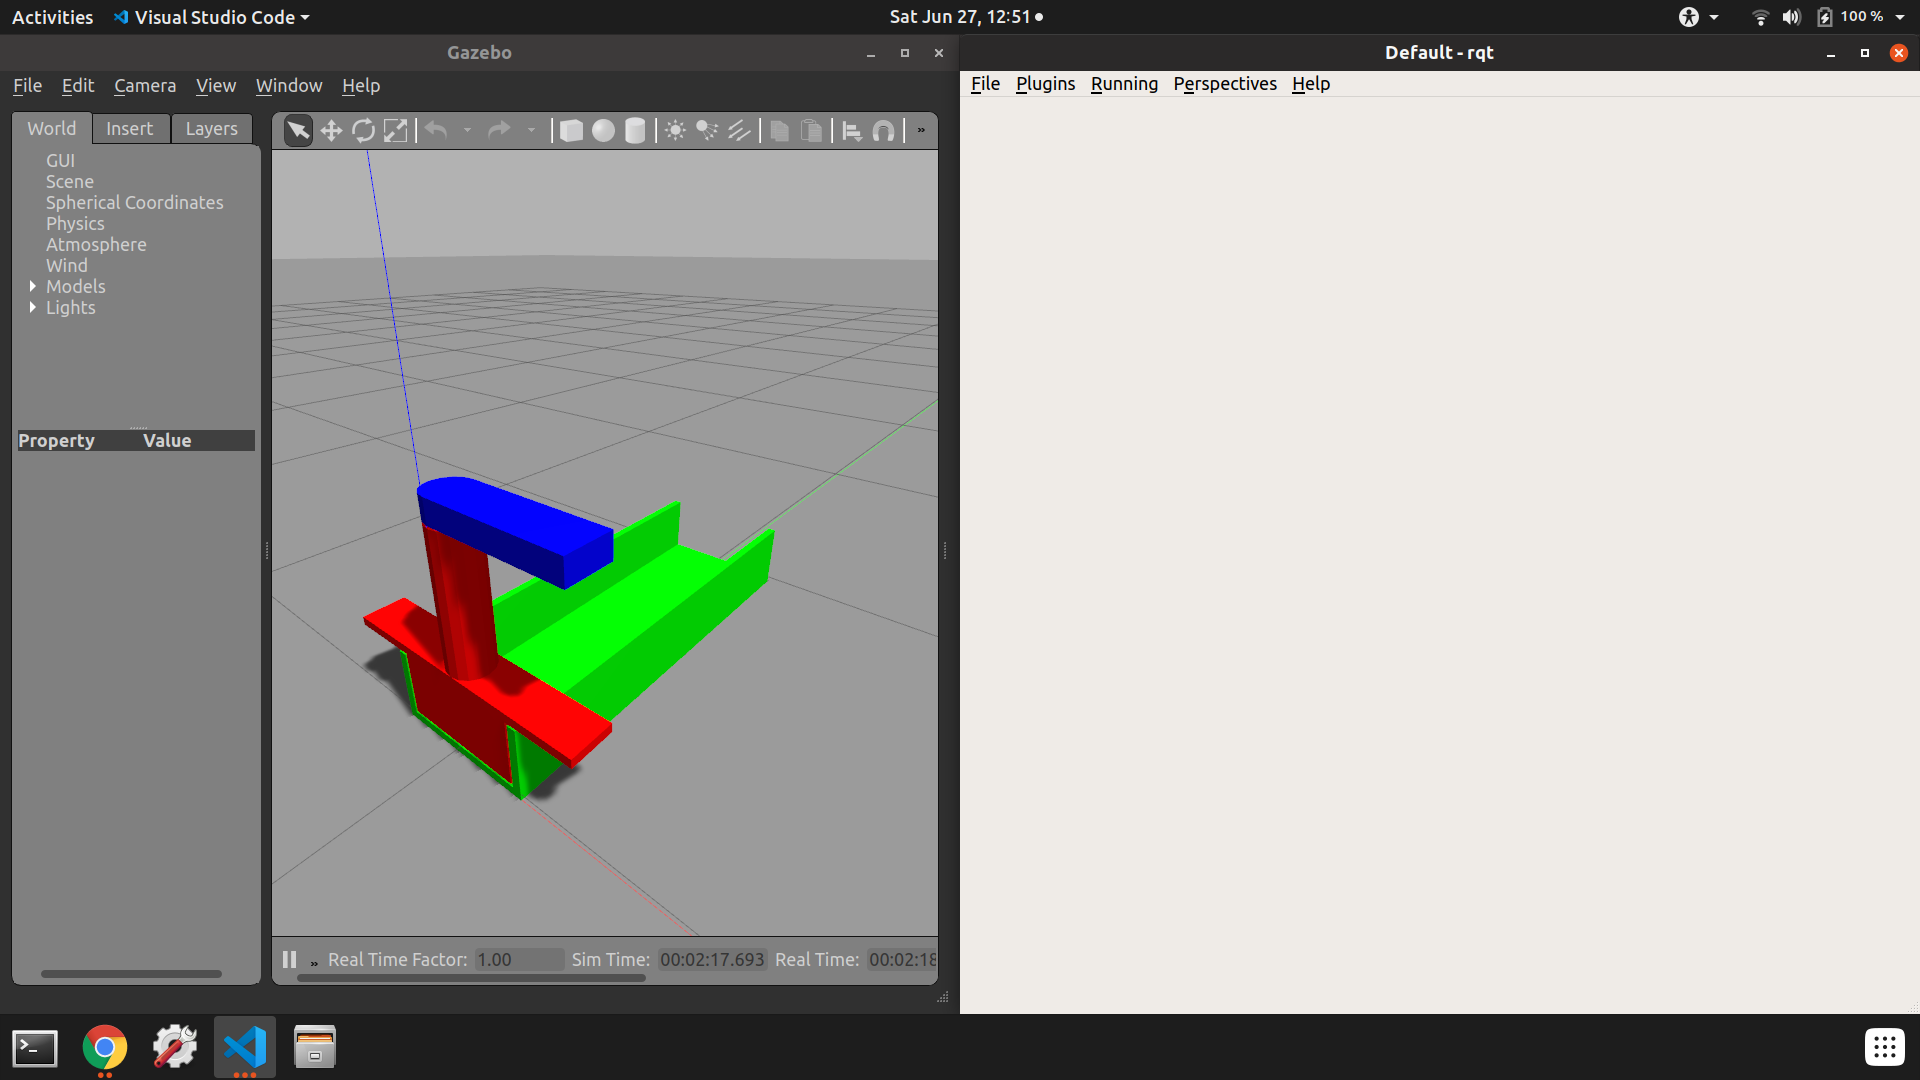
\includegraphics[width = \textwidth]{image_2.png}
            \end{figure}
            \item Plugins -- Topics -- Message Publisher.
            \begin{figure}[H]
                \center
                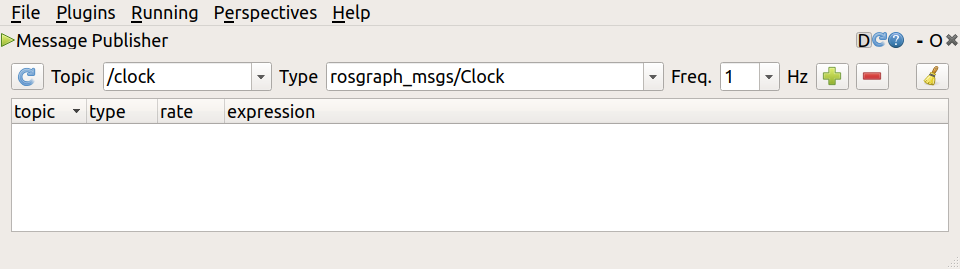
\includegraphics[width = \textwidth]{image_3.png}
            \end{figure}
            \item Add the following topics to the message publisher at 60 Hertz (use the + button). 
            \begin{itemize}
                \item \texttt{/j1\_controller/command}
                \item \texttt{/j2\_controller/command}
            \end{itemize}
            \begin{figure}[H]
                \center
                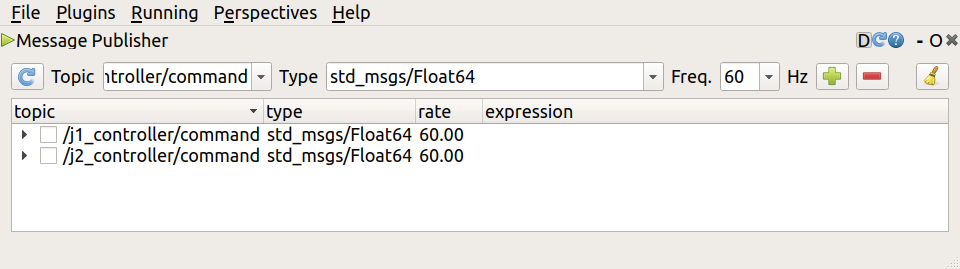
\includegraphics[width = \textwidth]{image_4.png}
            \end{figure}
            \item Click the small arrow beside the entry, change the data field from 0 to a sensible number,
            click the checkbox and see the robot move!
            \item You can control the robot using the topics mentioned above. You can get joint state information 
            from another topic. This is useful if you wish to write your own control algorithm or use a 
            package like ROS MoveIt. \textbf{Note:} If the revolute joint is behaving strangely at +3.14 and -3.14, change 
            the joint limits so that they are very clearly non-overlapping. The joint position controller gets confused if the 
            joint limits are overlapping.
            \item Now, let us tune the controller. Change the data field to $3.14\sin(\frac{i}{100})$. You should see the 
            joint oscillate between the extreme positions.
            \item In another terminal, run \texttt{rqt\_plot}.
            \item \begin{figure}[H]
                \center
                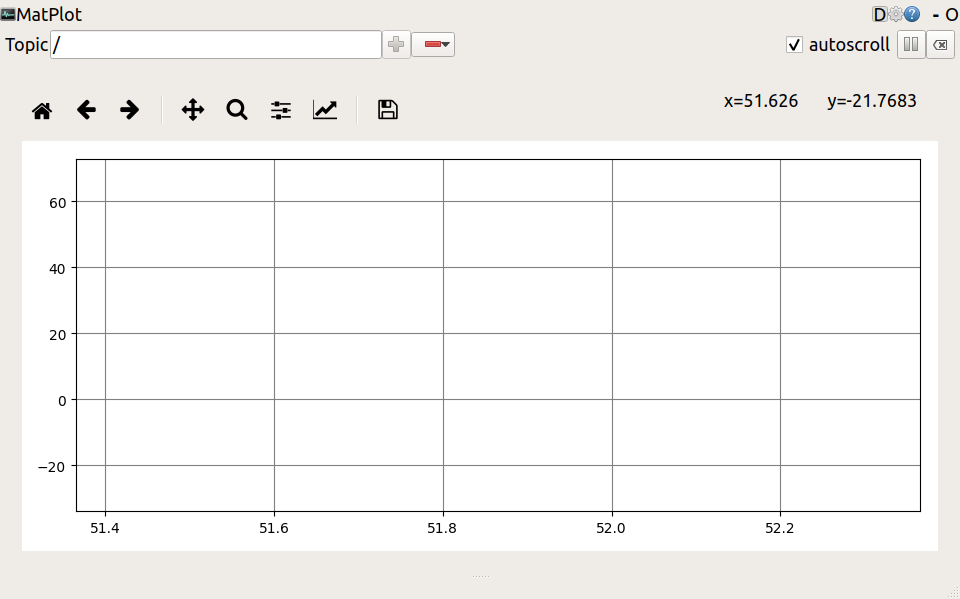
\includegraphics[width = \textwidth]{image_5.png}
            \end{figure}
            Add the following topics:
            \begin{itemize}
                \item \texttt{/j2\_controller/command}
                \item \texttt{/joint\_states/velocity[1]}
            \end{itemize}
            You should see a moving plot. 
            \item To tune the PIDs to optimize the response, go 
            back to \texttt{rqt\_gui}, minimize the Message Publisher and add Plugins -- Configuration -- 
            Dynamic Reconfigure.
            \begin{figure}[H]
                \center
                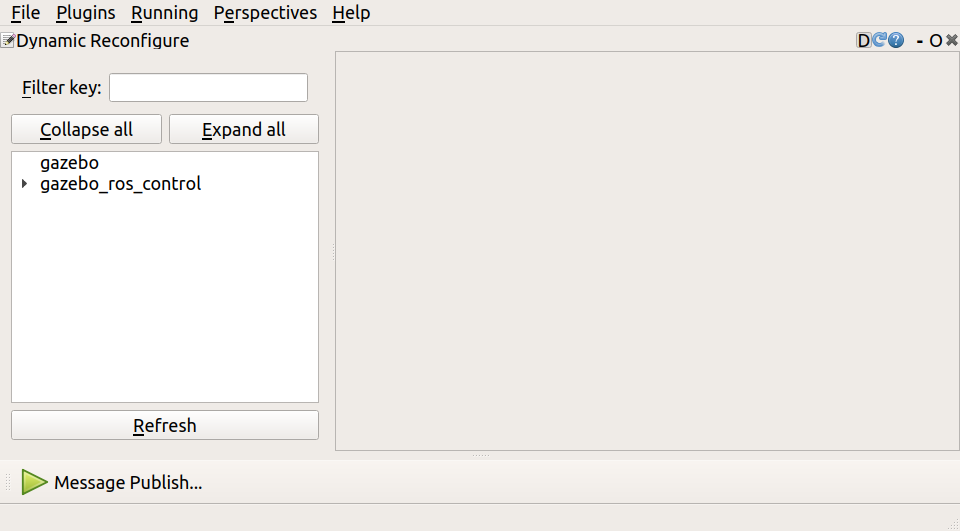
\includegraphics[width = \textwidth]{image_6.png}
            \end{figure}
            Add \texttt{gazebo\_ros\_control/pid\_gains/j2} to the display.
            \item \begin{figure}[H]
                \center
                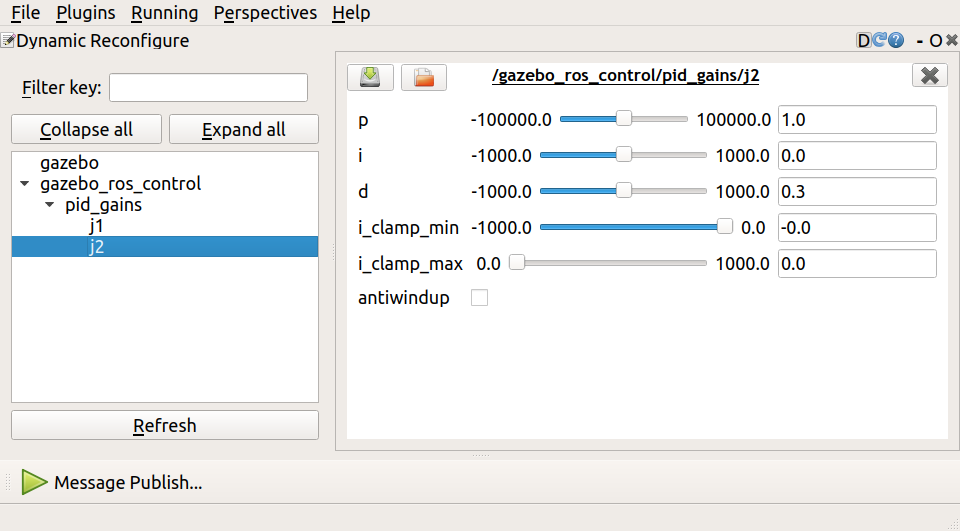
\includegraphics[width = \textwidth]{image_7.png}
            \end{figure}
            You can tune the PIDs. Tune it such that the curves match up -- but don't worry
            if you can't get it right. Manual PID tuning is a finicky thing. 
        \end{enumerate}
        \section{Looking ahead}
        Congratulations! You should be able to simulate simple robots using Gazebo and 
        ROS. Next, I recommend you learn how to integrate simulated sensors with the robot, 
        and make something simple, like a line follower. See \url{http://gazebosim.org/tutorials?tut=ros_gzplugins}
        for this. (I may or may not release a tutorial for this, depending on demand).
\end{document}